%%%%%%%%%%%%%%%%%%%%%%%%%%%%%%%%%%%%%%%%%
% Journal Article
% LaTeX Template
% Version 1.3 (9/9/13)
%
% This template has been downloaded from:
% http://www.LaTeXTemplates.com
%
% Original author:
% Frits Wenneker (http://www.howtotex.com)
%
% License:
% CC BY-NC-SA 3.0 (http://creativecommons.org/licenses/by-nc-sa/3.0/)
%
%%%%%%%%%%%%%%%%%%%%%%%%%%%%%%%%%%%%%%%%%
%----------------------------------------------------------------------------------------
%       PACKAGES AND OTHER DOCUMENT CONFIGURATIONS
%----------------------------------------------------------------------------------------
\documentclass[paper=letter, fontsize=12pt]{article}
\usepackage[english]{babel} % English language/hyphenation
\usepackage{amsmath,amsfonts,amsthm} % Math packages
\usepackage[utf8]{inputenc}
\usepackage{float}
\usepackage{lipsum} % Package to generate dummy text throughout this template
\usepackage{blindtext}
\usepackage{graphicx} 
\usepackage{xcolor}
\usepackage{caption}
\usepackage{subcaption}
\usepackage[sc]{mathpazo} % Use the Palatino font
\usepackage[T1]{fontenc} % Use 8-bit encoding that has 256 glyphs
\linespread{1.05} % Line spacing - Palatino needs more space between lines
\usepackage{microtype} % Slightly tweak font spacing for aesthetics
\usepackage[hmarginratio=1:1,top=32mm,columnsep=20pt]{geometry} % Document margins
\usepackage{multicol} % Used for the two-column layout of the document
%\usepackage[hang, small,labelfont=bf,up,textfont=it,up]{caption} % Custom captions under/above floats in tables or figures
\usepackage{booktabs} % Horizontal rules in tables
\usepackage{float} % Required for tables and figures in the multi-column environment - they need to be placed in specific locations with the [H] (e.g. \begin{table}[H])
\usepackage{hyperref} % For hyperlinks in the PDF
\usepackage{lettrine} % The lettrine is the first enlarged letter at the beginning of the text
\usepackage{paralist} % Used for the compactitem environment which makes bullet points with less space between them
\usepackage{abstract} % Allows abstract customization
\renewcommand{\abstractnamefont}{\normalfont\bfseries} % Set the "Abstract" text to bold
\renewcommand{\abstracttextfont}{\normalfont\small\itshape} % Set the abstract itself to small italic text
\usepackage{titlesec} % Allows customization of titles

\renewcommand\thesection{\Roman{section}} % Roman numerals for the sections
\renewcommand\thesubsection{\Roman{subsection}} % Roman numerals for subsections

\titleformat{\section}[block]{\large\scshape\centering}{\thesection.}{1em}{} % Change the look of the section titles
\titleformat{\subsection}[block]{\large}{\thesubsection.}{1em}{} % Change the look of the section titles
\newcommand{\horrule}[1]{\rule{\linewidth}{#1}} % Create horizontal rule command with 1 argument of height
\usepackage{fancyhdr} % Headers and footers
\pagestyle{fancy} % All pages have headers and footers
\fancyhead{} % Blank out the default header
\fancyfoot{} % Blank out the default footer

\lhead[C]{FCEFyN-UNC } % Custom header text
\rhead{
\includegraphics[scale=0.2]{header_unc.jpg}}
\fancyfoot[RO,LE]{\thepage} % Custom footer text
%----------------------------------------------------------------------------------------
%       TITLE SECTION
%----------------------------------------------------------------------------------------
\title{\bigskip \bigskip \bigskip \bigskip \vspace{-15mm}\fontsize{24pt}{10pt}\selectfont\textbf{ARQUITECTURA DE COMPUTADORAS \\}
\bigskip \bigskip \fontsize{18pt}{10pt}\selectfont\textbf{Trabajo Práctico 1 - ALU}} % Article title
\author{
\large
{\textsc{Casabella Martin, 39694763 }}\\[2mm]
\bigskip
  martin.casabella@alumnos.unc.edu.ar\\[2mm]
{\textsc{Morales Julian, 35046503 }}\\[2mm]
 jmorales@unc.edu.ar
%\thanks{A thank you or further information}\\ % Your name
%\normalsize \href{mailto:marco.torres.810@gmail.com}{marco.torres.810@gmail.com}\\[2mm] % Your email address
}
\date{}

%----------------------------------------------------------------------------------------
\begin{document}
\maketitle % Insert title
\thispagestyle{fancy} % All pages have headers and footers

\bigskip
\bigskip

\section{\textbf{Introducción}} \label{intro}
Para el primer trabajo práctico de la materia se realizó la implementación en FPGA de una Unidad Aritmética Lógica (ALU). Se desarrolló trabajando con la placa Basys 3 de digilent, y su FPGA Artix, utilizando el software Vivado 2018.2. 
El módulo posee un bus de datos parametrizable, junto con la longitud del código de operación, a fines de escalabilidad en el diseño y uso posterior en los siguientes trabajos.

\bigskip
\bigskip
\bigskip

\begin{figure}[H]
\centering
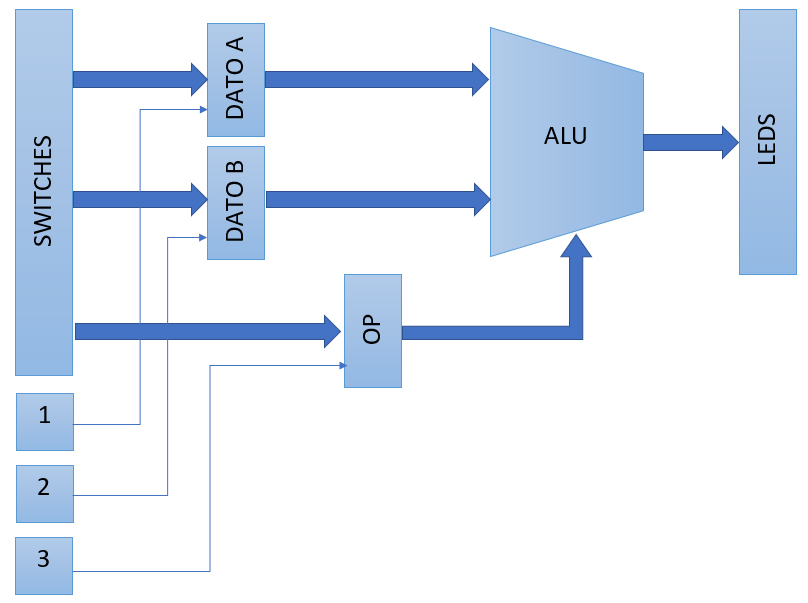
\includegraphics[scale=0.9, width=.6\textwidth]{alu.jpg}
\caption{\label{fig:alu}Diagrama de la ALU}
\end{figure}

\bigskip
\bigskip

La ALU soporta las siguientes operaciones, con los siguientes códigos:
\begin{table}[H]
\centering
\begin{tabular}{@{}ll@{}}
\toprule
Operación & Código \\ \midrule
ADD       & 100000 \\
SUB       & 100010 \\
AND       & 100100 \\
OR        & 100101 \\
XOR       & 100110 \\
SRA       & 000011 \\
SRL       & 000010 \\
NOR       & 100111 \\ \bottomrule
\end{tabular}
\caption{Operaciones de la ALU}
\label{operaciones}
\end{table}

\section{\textbf{Desarrollo}} \label{desarrollo_secc}

Para el desarrollo del módulo se definió una jerarquía de modulos conformada por el modulo de la ALU, integrado en un top level, como se muestra en la figura:

\begin{figure}[H]
\centering
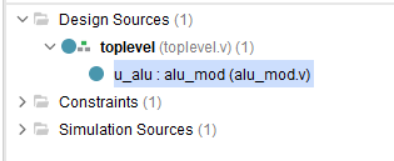
\includegraphics[scale=0.9, width=.6\textwidth]{modules.png}
\caption{Jerarquía de módulos}
\end{figure}

El módulo de la toplevel, esta conformado por los siguientes puertos y parametros:

\begin{itemize}
\item \textcolor{red}{parameter} $[BUS\_LEN -1 : 0]$ \textbf{BUS\_LEN}  : Parámetro que define el tamaño del bus 
\item \textcolor{olive}{input} $[BUS\_LEN -1 : 0]$ \textbf{i\_sw}  : Bus por donde el usuario ingresa ya sea un operando, o el opcode (switches físicos)
\item \textcolor{olive}{input} \textbf{i\_btnC} : Botón central que se pulsa para almacenar el opcode
\item \textcolor{olive}{input} \textbf{i\_btnL} : Botón izquierdo, que se pulsa para almacenar el operando 1 
\item \textcolor{olive}{input} \textbf{i\_btnR} : Botón derecho, que se pulsa para almacenar el operando 2
\item \textcolor{olive}{input} \textbf{i\_btnU} : Botón superior, asignado al reset del sistema
\item \textcolor{olive}{input}  \textbf{i\_clk}    : Clock de referencia sintetizado
\item \textcolor{olive}{output} $[BUS\_LEN -1 : 0 ]$ \textbf{o\_led} : Puerto de salida donde se mostrara el resultado (cableado a LEDs de la placa)

\end{itemize}


Para almacenar los valores ingresados se definieron dos registros $datoA$ y $datoB$, que mantienen los operandos, mientras que otro registro introducido $opcode$, almacena el código de operación ingresado. 
A su vez, se define un \textcolor{violet}{wire} que se le asigna a la instancia de la ALU para cablear el módulo top al registro del módulo de la ALU que almacena el resultado de la operación hecha.
El mismo, va a los LEDs, como se mencionó anteriormente.

Una vez definido el tamaño de BUS deseado, el módulo se centra en un bloque \textbf{\textcolor{cyan}{always}} que se ejecuta con cada flanco positivo del clock. Si se detecta que alguno de los dos elementos de
control están presionados (botón izquierdo o central) se almacena en el registro correspondiente el valor en los switchs.
Se encienden 3 LEDS asignados para indicar el ingreso con su respectiva secuencia, a modo indicativo.
Si el opcode es inválido, nada se visualiza en los LEDs. 
En cualquier otro momento, simplemente se copia el valor anterior de cada registro para mantenerlo guardado en el Flip-Flop.

Para el ingreso por pulsadores o botones, se realiza una detección de flanco, siendo normal cerrados los pulsadores de la placa. Para ello, se introduce un registro auxiliar, y se
testea el estado del mismo en relación al pulsador, para saber si realmente el usuario pulsó el botón. Vemos la lógica de la detección de flanco en la siguiente porción de código:
\begin{figure}[H]
\centering
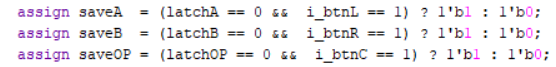
\includegraphics[scale=0.6]{buttons.png}
\end{figure}

\section{Test Bench}

A la hora de realizar los tests del módulo se elaboró un test bench o archivo de simulación que compruebe el funcionamiento de cada una de las operaciones programadas en la ALU.
Veamos el comportamiento del sistema en la siguiente figura:
\begin{figure}[H]
\centering
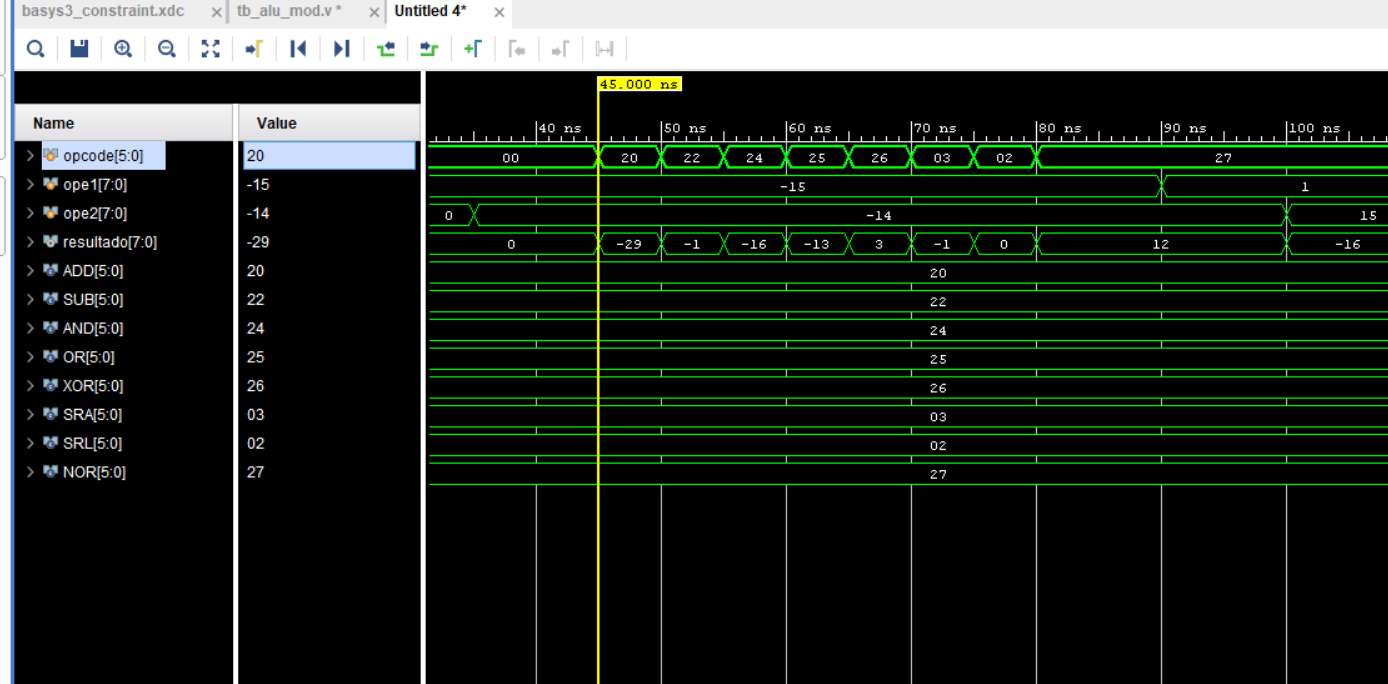
\includegraphics[scale=0.6]{testbench1.png}
\caption{Primer test bench realizado}
\end{figure}

Se ve al costado izquierdo de la figura, con representación decimal signada (tal y como se declararon los puertos de trabajo) los dos operandos ingresados.\\
A su vez, los parametros $ADD$, $SUB$, $AND$, $OR$, $XOR$, $SRA$, $SRL$, y $NOR$, internos al archivo de simulación, nos facilitan con la misma notación,
 el código de operación ingresado y por ende, la operación que se esta realizando en el instante de simulación dado.\\

Veamos con otros operandos distintos, y la misma secuencia de operaciones:\\

\begin{figure}[H]
\centering
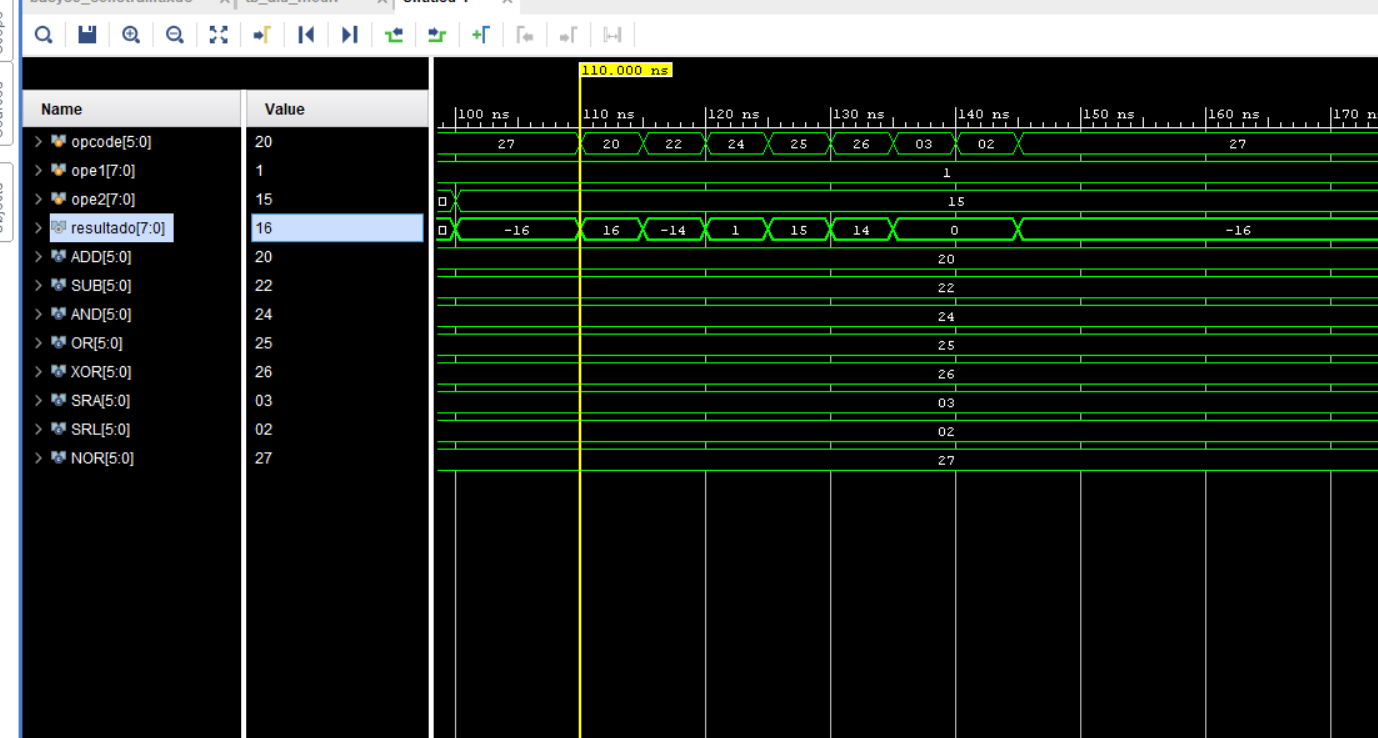
\includegraphics[scale=0.6]{testbench2.png}
\caption{Segundo test bench realizado}
\end{figure}


%\begin{thebibliography}{99}
%\bibitem [1]{stock} 
%James H. Stock, Mark  W. Watson, \textit{Forecasting inflation}, Journal of Monetary Economics 44 (1999) 293-335
%\end{thebibliography}


%----------------------------------------------------------------------------------------
%\end{multicols}
\end{document}




